\documentclass{article}

\usepackage[utf8]{inputenc}

\usepackage{nicefrac}
\usepackage{amssymb, amsmath, amsfonts}
\usepackage{amsthm}
\usepackage{tikz}
\usetikzlibrary{matrix,shapes,arrows}
\usepackage{pgfplots}
\usepgfplotslibrary{groupplots}
\usepackage[a4paper, margin=1in]{geometry}

\newtheorem{proposition}{Proposition}
\newtheorem{theorem}{Theorem}
\newtheorem{definition}{Definition}
\newtheorem{lemma}{Lemma}
\newtheorem{conjecture}{Conjecture}
\newtheorem{corollary}{Corollary}
\newtheorem{remark}{Remark}
\newtheorem{assumption}{Assumption}

\newlength\figureheight
\newlength\figurewidth
\setlength\figureheight{8cm}
\setlength\figurewidth{14cm}

\newcommand{\tikzdir}[1]{tikz/#1.tikz}
\newcommand{\inputtikz}[1]{\input{\tikzdir{#1}}}

\DeclareMathOperator*{\argmin}{arg\; min}     % argmin
\DeclareMathOperator*{\argmax}{arg\; max}     % argmax
\DeclareMathOperator*{\tr}{tr}     % trace
\DeclareMathOperator{\Cov}{Cov}
\DeclareMathOperator{\logdet}{log\;det}

\title{EE3011 Modeling and Control\\Quiz 3}
\date{}
\begin{document} \maketitle

\begin{enumerate}
\item Find the magnitude and phase responses of the following transfer function
  \[
    G(s) = \frac{s-1}{s+1}.
  \]
  Compute the steady-state responses to sinusoid $r(t) = 2\sin(t+30^\circ)$.

  \bf{Solution:}
\newpage

\item Sketch the Bode plots for the following transfer function
  \[
    G(s) = \frac{10(s+50)}{s(s+5)}.
  \]
  \bf{Solution:}
\begin{figure}[h]
\centering
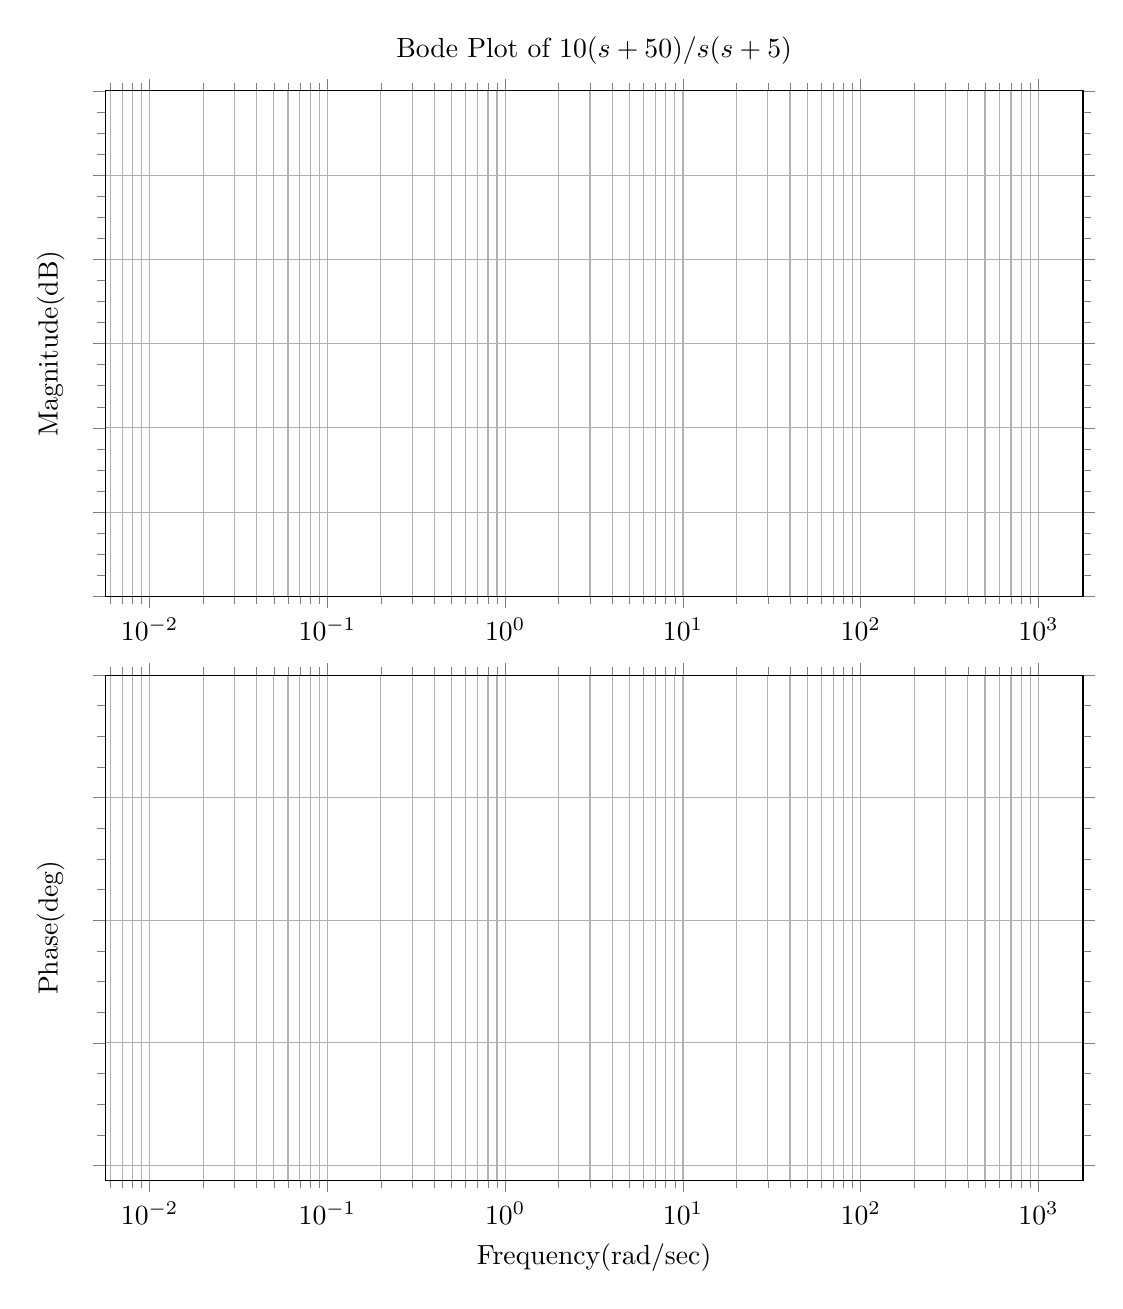
\begin{tikzpicture}
\begin{groupplot}[group style={group size=1 by 2}]
\nextgroupplot[
title={Bode Plot of $10(s+50)/s(s+5)$},
ylabel={Magnitude(dB)},
xmin=0.0056234132519035, xmax=1778.27941003892,
ymin=-40, ymax=80,
xmode=log,
width=\figurewidth,
height=\figureheight,
tick align=outside,
xmajorgrids,
yticklabels={,,,,,,},
xminorgrids,
minor y tick num=3,
yminorticks=true,
x grid style={white!69.019607843137251!black},
ymajorgrids,
y grid style={white!69.019607843137251!black}
]
\nextgroupplot[
xlabel={Frequency(rad/sec)},
ylabel={Phase(deg)},
ytick = {0,22.5,45,67.5,90},
xminorgrids,
minor y tick num=3,
yticklabels={,,,,},
xmin=0.0056234132519035, xmax=1778.27941003892,
ymin=-2.74288237589232, ymax=90,
xmode=log,
width=\figurewidth,
height=\figureheight,
tick align=outside,
xmajorgrids,
xminorgrids,
x grid style={white!69.019607843137251!black},
ymajorgrids,
y grid style={white!69.019607843137251!black}
]
\end{groupplot}

\end{tikzpicture}

\end{figure}
  
\end{enumerate}

\end{document}
%%% Local Variables:
%%% TeX-command-default: "Latexmk"
%%% End:
